\section{A Generalized Basic KAC Construction}
\label{sec:general}

In this section, we present a a generalized basic KAC construction. The essential idea is to run $n_A$ parallel instances of the basic scheme parameterized by $n_B$ number of classes, so that the overall system can handle as many as $n=n_A\times n_B$ data classes. Each of these instances share the same set of public parameters, but use their own set of private and public keys. This leads to a trade-off between the overhead for various system parameters. 

\subsection{The Construction}
\label{subsec:two-tier}

We present the construction for generalized KAC in this section. The construction uses techniques similar to the generalized broadcast encryption scheme proposed in \cite{boneh2005collusion}. The generalization in \cite{boneh2005collusion} trades off the ciphertext size with the public key size. Our scheme, on the other hand, trades off the public parameter size with the public key size and the aggregate key size, while still maintaining constant ciphertext overhead.\\

\noindent \textbf{SetUp}$(1^{\lambda},n_B)$: Randomly pick $\alpha \in \mathbb{Z}_q$. Output the system parameter as $param = (P,Q,Y_{P,\alpha,n_B},Y_{Q,\alpha,n_B}))$. Discard $\alpha$. \\

\noindent \textbf{KeyGen}($n_A$): Randomly pick $\gamma_{1},\cdots,\gamma_{n_A} \in \mathbb{Z}_q$. Let $msk_j=\gamma_j$, $PK^1_j=\gamma_{j}P$ and $PK^2_j=\gamma_{j}Q$ for $1\leq j \leq n_A$. Set the master secret key $msk=(msk_1,\cdots,msk_{n_A})$. Set $PK^1=(PK^1_1,\cdots,PK^1_{n_A})$ and $PK^2=(PK^2_1,\cdots,PK^2_{n_A})$. Finally, set the public key $PK=(PK^1,PK^2)$ and output the tuple $(msk,PK)$.\\

\noindent \textbf{Encrypt}$(PK,i,\mathcal{M})$: Compute $a_i=\lceil i/n_B\rceil$ and $b_i=i \text{ mod } B$. Randomly choose $t\in\mathbb{Z}_q$ and output the ciphertext $\mathcal{C}$ as 
 \begin{equation}
 \mathcal{C}=(c_1,c_2,c_3)=(tQ,t(PK^{2}_{a}+Q_{b}),\mathcal{M}.{e}(P_n,tQ_1)) \nonumber
 \end{equation} 

\noindent \textbf{Extract}$(msk,\mathcal{S})$: For the subset of class indices $\mathcal{S}$ and $1\leq a \leq n_A$, define
\begin{eqnarray}
 \mathcal{S}_{a}&=&\{i|i\in\mathcal{S},\lceil i/n_B\rceil=a\} \nonumber\\
 \mathcal{S}'_a&=&\{b_i=i\text{ mod }n_B|i\in\mathcal{S}_{a}\}\nonumber
\end{eqnarray}
\noindent Next, for $1\leq a \leq n_A$, compute
\begin{equation}
 K^{a}_{\mathcal{S}} = {msk_{a}}\sum_{b\in\mathcal{S}'_a}P_{n+1-b} \nonumber
\end{equation}
\noindent Note that this is indirectly equivalent to setting $K^{a}_{\mathcal{S}}$ to $\sum_{b\in\mathcal{S}'_a}\alpha^{n+1-b}PK^{1}_a$. Finally, output 
\begin{equation}
 K_{\mathcal{S}} = (K^{1}_{\mathcal{S}},\cdots,K^{n_A}_{\mathcal{S}})\nonumber
\end{equation}
\noindent Note that the the aggregate key now consists of $n_A$ elements.\\

\noindent \textbf{Decrypt}$(\mathcal{C},i,K_{\mathcal{S}},\mathcal{S})$: If $i\notin\mathcal{S}$, output $\bot$. Otherwise, compute $a_i=\lceil i/n_B\rceil$ and $b_i=i \text{ mod } B$ and set: 
 \begin{eqnarray} 
 A_{\mathcal{S}}&=&\sum_{(b\in\mathcal{S}'_{a_i},b\neq b_i}P_{n+1-b_i+b} \nonumber \\
 B_{\mathcal{S}}&=&\sum_{(b\in\mathcal{S}'_{a_i}}P_{n+1-b} \nonumber  
 \end{eqnarray} 
 \noindent Return the decrypted message $\hat{\mathcal{M}}$ as:
 \begin{equation}
  \hat{\mathcal{M}}=c_3.\frac{{e}(K^{a_i}_{\mathcal{S}}+A_{\mathcal{S}},c_1)}{{e}(B_{\mathcal{S}},c_2)}\nonumber
 \end{equation} 
\noindent Correctness of the algorithm may be easily proved similarly as in Section \ref{subsec:construction1}. Finally, we note that setting $n_A=1$ and $n_B=n$ gives the basic construction of Section \ref{subsec:construction1}. 


\subsection{Performance and Efficiency}
\label{subsec:perf_twotier}

The choice of $n_A$ and $n_B$ play an important role in system performance. As is clear from the construction, the ciphertext always consists of a constant number of group elements. The public parameter comprises of $n_B$ group elements, while the aggregate key as well as the public key consist of $n_A$ group elements each. Thus choosing a smaller value of $n_B$ is useful for applications requiring low overhead aggregate keys. However, choosing $n_A=n_B=\sqrt{n}$ minimizes overall system overhead combining all parameters.

\textbf{We present the simulation studies with different values of $n_A$ and $n_B$ here}.

% We look at the performance of the general KAC construction from the perspective of both parties involved - the data owner sharing her data and an user accessing the shared data. From the data owner's perspective, each superclass comprises of a basic KAC module parameterized with $n$, with constant size public, private and authentication keys. The encryption process can be speeded up using similar caching techniques described in Section \ref{subsec:perf_basic}. From the user's perspective, the system is an ensemble of basic KAC units - one per superclass. For a user willing to access data from $k$ data owners, the aggregate key and authentication keys have size linear in $k$. It seems difficult to do better than this while maintaining data isolation and privacy for each data owner. As in encryption, the decryption process can also be expedited using appropriate caching techniques. It is important to note that the public $param$, which essentially forms the fundamental basic for the security of the general KAC, is a function of $n$ only, and does not depend on the number of users $M$ registered in the system.
% 
% An important aspect of this construction is to decide on an appropriate value for $n$. Keeping a small $n$ value reduces the size of the public parameter. But then a data owner with a large number of data classes $N$ would have to register with $\lceil N/n \rceil$ public, private and authentication key sets, which may not be desirable. Thus there exists a trade-off in using smaller and larger values of $n$ in this scheme. 

% It is important to note that the security of the system depends on the $(n,n)$-BDHE assumption, as we show next.

% \begin{figure*}
% \centering
% \captionsetup{font=scriptsize}
% 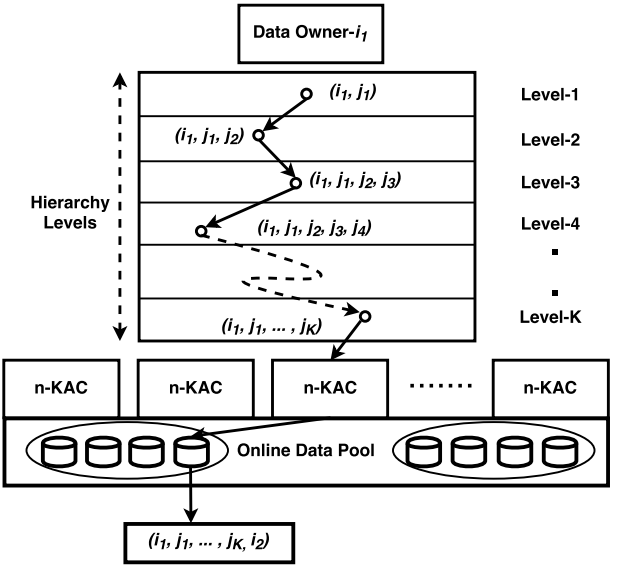
\includegraphics[scale=0.4]{Figs/Hierarchical.png}
% \caption{Hierarchical KAC}
% \label{fig:K-tier}
% \end{figure*}

\subsection{Semantic Security of General KAC}
\label{subsec:security_twotier}

For the non-adaptive CPA security of the generalized KAC construction, we state the following theorem.

\begin{Theorem}
\label{th:twotierCPA}
Let $\mathbb{G}_1$ and $\mathbb{G}_2$ be bilinear elliptic curve subgroups of prime order $q$. For any pair of positive integers $n',n (n'>n)$, the generalized KAC is $(\tau,\epsilon,n')$ CPA secure if the asymmetric decision $(\tau,\epsilon,n)$-BDHE assumption holds in $(\mathbb{G}_1,\mathbb{G}_2)$.
\end{Theorem}

\noindent The proof of this theorem is very similar to the proof of Theorem \ref{th:basicCPA} and is hence avoided.

% \noindent{\textit{Proof:}} Let $\mathcal{A}$ be a $\tau$-time adversary such that $|Adv_{\mathcal{A},n'}-\frac{1}{2}| > \epsilon$ for a two-tier KAC system parameterized with a given $n$. We build an algorithm $\mathcal{B}$ that has advantage at least $\epsilon$ in solving the $(n,n)$-BDHE problem in $(\mathbb{G}_1,\mathbb{G}_2)$. Algorithm $\mathcal{B}$ takes as input a random $(n,n)$-BDHE challenge $(I'=(H',P,Q,Y_{P,\alpha,n},Y_{Q,\alpha,n}),Z')$ (where $Z'$ is either ${e}(P_{n+1},H')$ or a random value in $\mathbb{G}_T$), and proceeds as follows.\\
% 
% \noindent \textbf{Init:} $\mathcal{B}$ runs $\mathcal{A}$ and receives the set $\mathcal{S}$ of ciphertext classes that $\mathcal{A}$ wishes to be challenged on. $\mathcal{B}$ then randomly chooses a ciphertext class $(a,b)\in\mathcal{S}$.\\
% 
% \noindent \textbf{SetUp}: As discussed before, $\mathcal{B}$ should generate the public $param$, public key $PK$, the authentication key $U$, and the aggregate key $K_{\overline{\mathcal{S}}}$ and provide them to $\mathcal{A}$. They are generated as follows.
% %  \vspace{-0.6mm}
%  \begin{itemize}
%   \item $param$ is set as $(P,Q,Y_{P,\alpha,n},Y_{Q,\alpha,n})$.
%   \item $msk^{a}$ is set as some $u$ randomly chosen from $\mathbb{Z}_q$.
%   \item Set $PK^{a}=(PK^{a}_1,PK^{a}_2)$, where $PK^{a}_1$ and $PK^{a}_2$ are computed as $uP - P_{b}$ and $uQ-Q_{b}$ respectively.
%   \item $K^{a}_{\overline{\mathcal{S}}}$ is set as $\sum_{(a,j_2)\notin\mathcal{S}}({u}P_{n+1-j_2}-(P_{n+1-j_2+b}))$.   
%   \item Choose a random $t\in \mathbb{Z}_q$, and set $U^{a}=tQ$.
%  \end{itemize}
%  
% \noindent Since $P$, $Q$ $\alpha$, $U^{a}$ and the $u$ values are chosen uniformly at random, \emph{the public parameters and the public key have an identical distribution to that in the actual construction}. Also note that providing $\mathcal{A}$ with the aggregate key or the authentication key is unnecessary since they do not impart any information about an encrypted message in the class $(a,b)$. \\
% 
% \noindent \textbf{Challenge}: As before, to generate the challenge, $\mathcal{B}$ picks at random two messages $m_0$ and $m_1$ from the set of possible plaintext messages belonging to class $(a,b)$. She randomly picks $b\in\{0,1\}$, and sets the challenge as $(\mathcal{C},m_0,m_1)$, where $\mathcal{C}=(H'-U^{a},uH',m_b.Z')$. We claim that when $Z'={e}(P_{n+1},H')$ (i.e. the input to $\mathcal{B}$ is a valid $(n,n)$-BDHE tuple), then $(\mathcal{C},m_0,m_1)$ is a valid challenge to $\mathcal{A}$ as in a real attack. To see this, we write $H'=t'Q$ for some unknown $t'\in\mathbb{Z}_q$. Then we have $H'-U=rQ$ for some unknown $r=t-t'$, and $uH'$ = $t'(uQ)$ = $t'(uQ-{Q_{b}}+Q_{b})$ = $t'(PK^{a}_2+Q_{b})$. Finally, $m_b.Z'=m_b{e}(P_{n+1},t'Q)$. Thus, by definition, $\mathcal{C}$ is a valid encryption of the message $m_b$ in class $(a,b)$ and hence, $(\mathcal{C},m_0,m_1)$ is a valid challenge to $\mathcal{A}$.\\
% 
% \noindent \textbf{Guess}: The adversary $\mathcal{A}$ outputs a guess $b'$ of $b$. If $b' = b$, $\mathcal{B}$ outputs $0$ (indicating that $Z' = {e}(P_{n+1},H')$). Otherwise, it outputs $1$ (indicating that $Z'$ is a random element in $\mathbb{Z}_T$).\\
%  
% A similar analysis as in Section \ref{subsec:proof_basic} establishes that $\mathcal{B}$ has advantage at least $\epsilon$ in solving the $(n,n)$-BDHE problem in $(\mathbb{G}_1,\mathbb{G}_2)$. This concludes the proof of Theorem \ref{th:twotierCPA}.
% 
% It is important to note that in a practical environment, any data sharing scheme is expected to support a hierarchical organization of data, where different users are given access to different levels of the data. For example, consider an online data pool on the cloud storing an organization's data. The organization (which owns the data) would like to delegate access rights to this data among its employees. Different employees may be given access to different levels of this data depending on their respective credentials and designation. The most common solution to this is to have a pre-defined hierarchical framework for organizing the data, and have keys at different levels of the hierarchy. As pointed out in our previous discussion, highly irregular data access patterns from multiple users could compromise the efficiency of such a hierarchical system by potentially blowing up the size of the key to be shared. Since key aggregation allows us to combine the decryption rights to multiple data classes into a single constant-sized entity, it seems KAC could be the most efficient solution even in this scenario. However, we show next via a small example that the generalized KAC in its original form may not be able to tackle this problem in the most efficient manner.   
% 
% Although the generalized KAC is highly scalable and efficient, it has a drawback in the sense that it fails to support hierarchical organization of data within a single data owner system. Consider the scenario in which a data owner would like to have two distinct folders, namely $F_1$ and $F_2$, that are meant to be accessed by separate user groups. In the generalized KAC framework, she must then have different public, private and authentication keys for these folders. Now if she were to delegate decryption rights to some user for a subset of files both these folders, she would need to provide two aggregate keys, one for each folder. This is because the generalized KAC does not allow her to aggregate these two keys into a single key. If she wants to provide a single aggregate key for both the folders, she would need to have another aggregate system in place to combine these two individual keys. This process is cumbersome and becomes difficult to maintain as the number of hierarchy levels grow. The same disadvantage also persists with the KAC proposed in \cite{chu2014key}. However, since data hierarchy is extremely common in file-based storage systems, we must adopt KAC so as to be able to provide the advantage of key aggregation for any arbitrarily complex hierarchical structure, without the data owner having to worry about the internal details of the aggregation. The modified KAC infrastructure must now support key aggregation at various levels of the hierarchy, while using the same security guarantees provided the fundamental single data owner KAC. This motivates the introduction of an augmented version of the general KAC in the next section, which we refer to as the \emph{hierarchical} KAC.   




% In this section, we focus on building an efficiently extensible version of our proposed scheme that allows an user to economically increase the number of ciphertext classes while registering a new public key-private key pair. We adopt the idea presented in \cite{boneh2005collusion} to develop a hierarchical structure that has multiple instances (say $M$) of the original scheme running in parallel. Each such instance in turn provides \emph{locally aggregate keys} for $n$ ciphertext sub-classes. Each ciphertext class thus now has a double index $(a,b)$ where $1\leq a \leq M$ and $1\leq b \leq n$. This allows the overall setup to handle $n=Mn$ classes. However, it is important to note that all the instances can use the same public parameters. This interaction among the instances helps to largely improve performance. We further point out that while in \cite{boneh2005collusion}, the two-tier construction offers a trade-off between the public parameter size and the ciphertext size, our 
% two-tier scheme actually reduces the public parameter size without compromising on the size of the ciphertext. Further, addition of a single new key increases the number of classes only by $n$ and not by $n$. Setting $n\ll n$ thus achieves significant improvement in performance over the existing proposal.


% \subsection{The Construction of the Two-tier KAC}
% \label{subsec:construction2}
% 
% Let $n$ be a fixed positive integer. Our proposed $n$-two-tier key-aggregate encryption scheme over elliptic curve subgroups is as described below. It may be noted that the bilinear additive elliptic curve sub-group $\mathbb{G}$ and the multiplicative group $\mathbb{G}_T$, as well as the pairing $\hat{e'}$ are the same as in the basic scheme. The algorithm sets up $M=\lfloor n/n\rfloor$ instances of the basic scheme, each of which handles $n$ ciphertext classes. The original scheme is thus a special case of the extended scheme with $M=1$ and $n=n$.
% 
% 
% \begin{enumerate}
%  \item \textbf{Setup}$(1^{\lambda},n)$: Randomly pick $\alpha \in \mathbb{Z}_q$. Compute $P_i$ = ${\alpha^{i}}P \in \mathbb{G}$ for $i = 1,\cdots,n,n+2,\cdots,2n$. Output the system parameter as $param$ = $(P,P_1,\cdots,P_{n},P_{n+2},\cdots,P_{2n})$. The system randomly chooses a secret parameter $t \in \mathbb{Z}_q$ which is not made public. It is only known to data owners with credentials to control client access rights.
%  \item \textbf{Keygen}(): Pick $\gamma_1,\gamma_2,\cdots,\gamma_{M} \in \mathbb{Z}_q$, output the public and master-secret key pair: $PK$=$({pk}_1,pk_{2},\cdots,pk_{M})$=$(\gamma_1P,\gamma_2P,\cdots,\gamma_{M}P)$, and $msk$=$(\gamma_1,\gamma_2,\cdots,\gamma_{M})$.
%  \item \textbf{Encrypt}$(pk_{a},(a,b),m)$: For a message $m \in \mathbb{G}_T$ and an index $(a,b) \in \{1,2,\cdots,M\}\times\{1,2,\cdots,n\}$, randomly choose $r\in\mathbb{Z}_q$ and let $t'=t+r \in\mathbb{Z}_q$. Then compute the ciphertext $\mathcal{C}$=$(rP,t'{(pk_{a}+P_{b})},m.\hat{e'}(P_{n},t'P_1))$ = $(c_1,c_2,c_3)$.
%  \item \textbf{Extract}$(msk=\gamma,\mathcal{S})$: For the set $\mathcal{S}$ of indices $(\hat{a},j_2)$ the aggregate key is computed as $K_{\mathcal{S}}$ = $(k^{1}_{\mathcal{S}},k^{2}_{\mathcal{S}},\cdots,k^{M}_{\mathcal{S}})$, where $k^{i}_{\mathcal{S}}$ = $\sum_{(i,j_2)\in\mathcal{S}}{\gamma_{1}}P_{n+1-j_2}$. The dynamic access control parameter $U$ is computed as $tP$. Thus the net aggregate key is $(K_{\mathcal{S}},U)$ which is transmitted via a secure channel to users that have access rights to $\mathbb{S}$. Note that  $k^{\hat{a}}_{\mathcal{S}}=\sum_{(\hat{a},j_2)\in\mathcal{S}}\alpha^{n+1-j}pk_{\hat{a}}$ for $\hat{a}=1,2,\cdots,M$. 
%  \item \textbf{Decrypt}$(K_{\mathcal{S}}, U, \mathcal{S},(a,b),\mathcal{C}=\{c_1,c_2,c_3\})$: If $(a,b)\notin\mathcal{S}$, output $\bot$. Otherwise return the message $\hat{m}$ = $c_3\frac{\hat{e'}(k^{a}_{\mathcal{S}}+\sum_{(a,j_2)\in\mathcal{S},j_2\neq b}P_{n+1-j_2+b},U+c_1)}{\hat{e'}(\sum_{(a,j_2)\in\mathcal{S}}P_{n+1-j_2},c_2)}$. 
% \end{enumerate}
% 
% The proof of correctness for the two-tier scheme is presented below.
% 
% \begin{scriptsize}
% \begin{equation}
% \begin{split}
%  \hat{m} &= c_3\frac{\hat{e'}(k^{a}_{\mathcal{S}}+\sum_{(a,j_2)\in\mathcal{S},j_2\neq b}P_{n+1-j_2+b},U+c_1)}{\hat{e'}(\sum_{(a,j_2)\in\mathcal{S}}P_{n+1-j_2},c_2)}\\
%   &= c_3\frac{\hat{e'}(\sum_{(a,j_2)\in \mathcal{S}}{\gamma_{a}}P_{n+1-j_2} + \sum_{(a,j_2)\in\mathcal{S},j_2\neq b}P_{n+1-j_2+b},t'P)}{\hat{e'}(\sum_{(a,j_2)\in\mathcal{S}}P_{n+1-j_2},t'(pk_{a}+P_{b})}\\
% %   &= c_3\frac{\hat{e'}(\sum_{(a,j_2)\in \mathcal{S}}{\gamma_{a}}P_{n+1-j_2},t'P)\hat{e'}(\sum_{(a,j_2)\in\mathcal{S}}(P_{n+1-j_2+b})-P_{n+1},t'P)}{\hat{e'}(\sum_{(a,j_2)\in\mathcal{S}}P_{n+1-j_2},t'pk_{a})\hat{e'}(\sum_{(a,j_2)\in\mathcal{S}}P_{n+1-j_2},t'P_{b})}\\
%   &= c_3\frac{\hat{e'}(\sum_{(a,j_2)\in\mathcal{S}}P_{n+1-j_2+b},t'P)}{\hat{e'}(P_{n+1},t'P)\hat{e'}(\sum_{(a,j_2)\in\mathcal{S}}P_{n+1-j_2},t'P_{b})}\\
%   &= c_3\frac{\hat{e'}(\sum_{(a,j_2)\in\mathcal{S}}P_{n+1-j_2+b},t'P)}{\hat{e'}(P_{n+1},t'P)\hat{e'}(\sum_{(a,j_2)\in\mathcal{S}}P_{n+1-j_2+b},t'P)}\\
%   &= m\frac{\hat{e'}(P_{n},t'P_1)}{\hat{e'}(P_{n+1},t'P)}\\
%   &= m
% \end{split}  
% \end{equation}
% \end{scriptsize}
% 
% 
% \subsection{Semantic Security of the Two-tier KAC}
% \label{subsec:proof_general}
% 
% \subsubsection{The Reduced Two-tier Scheme:}
% 
% We define a reduced version of the two-tier encryption scheme. We note that the ciphertext $\mathcal{C}=(c_1,c_2,c_3)$ output by the $Encypt$ operation essentially embeds the value of $m$ in $c_3$ by multiplying it with $\hat{e'}(P_{n},tP_1)$. Consequently, the security of our proposed scheme is equivalent to that of a \emph{reduced} two-tier key-aggregate encryption scheme that simply uses the reduced ciphertext $(c_1,c_2)$, the aggregate key $K_{\mathcal{S}}$ and the dynamic access parameter $U$ to successfully transmit and decrypt the value of $\hat{e'}(P_{n},t'P_1)=\hat{e'}(P_{n+1},t'P)$. We prove the semantic security of this \emph{reduced scheme} parameterized with a given number of ciphertext classes $n$ for each instance, which also amounts to proving the semantic security of our original encryption scheme for the same number of ciphertext classes. Note that the proof of security is independent of the number of instances $M$ that run in parallel.
% 
% \subsubsection{The Adversarial Model:} We make the following assumptions about the adversary $\mathcal{A}$:
% 
% \begin{enumerate}
%  \item The adversary has the aggregate key that allows her to access any ciphertext class other than those in the target subset $\mathcal{S}$, that is, she possesses $K_{\overline{\mathcal{S}}}$.
%  \item The adversary has access to the public parameters $param$ and $PK$, and also possesses the dynamic access parameter $U$.
% %  \item The adversary is authorized and and hence 
% \end{enumerate}
% 
% 
% \subsubsection{The Security Proof:}
% 
% The security proof presented here uses the first complexity assumption stated in \ref{subsubsec:asm_1}. Let $\mathbb{G}$ be a bilinear elliptic curve subgroup of prime order $q$. For any pair of positive integers $n,n' (n'>n)$ our proposed $n$-two-tier reduced key-aggregate encryption scheme over elliptic curve subgroups is $(\tau,\epsilon,n')$ semantically secure if the decision $(\tau,\epsilon,n)$-BDHE assumption holds in $\mathbb{G}$. We now prove this statement below.
% 
% \textbf{\noindent{Proof:}} Let for a given input $n'$, $\mathcal{A}$ be a $\tau$-time adversary that has advantage greater than $\epsilon$ for the \emph{reduced scheme} parameterized with a given $n$. We build an algorithm $\mathcal{B}$ that has advantage at least $\epsilon$ in solving the $n$-BDHE problem in $\mathbb{G}$. Algorithm $\mathcal{B}$ takes as input a random $n$-BDHE challenge $(P,H,Y_{(P,\alpha,n)},Z)$ where $Z$ is either $\hat{e'}(P_{n+1},H)$ or a random value in $\mathbb{G}_T$. Algorithm $\mathcal{B}$ proceeds as follows.
% 
% \begin{enumerate}
%  \item \textbf{Init:} Algorithm $\mathcal{B}$ runs $\mathcal{A}$ and receives the set $\mathcal{S}$ of ciphertext classes that $\mathcal{A}$ wishes to be challenged on. For each ciphertext class $(a,b)\in\mathcal{S}$, $\mathcal{B}$ performs the \textbf{SetUp}-$\mathbf{(a,b)}$, \textbf{Challenge}-$\mathbf{(a,b)}$ and \textbf{Guess}-$\mathbf{(a,b)}$ steps. Note that the number of iterations is polynomial in $|S|$. 
%  
%  \item \textbf{SetUp}-$\mathbf{(a,b)}$: $\mathcal{B}$ should generate the public $param$, public key $PK$, the access parameter $U$, and the aggregate key $K_{\overline{\mathcal{S}}}$. For the iteration corresponding to ciphertext class $(a,b)$, they are generated as follows.
%  \begin{itemize}
%   \item $param$ is set as $(P,Y_{P,\alpha,n})$.
%   \item Randomly generate $u_1,u_2,\cdots,u_{M} \in \mathbb{Z}_q$. Then, set $PK$= $(pk_1,pk_2,\cdots,pk_{M})$, with $pk_{\hat{a}}$ = $u_{\hat{a}}P - P_{b}$ for $\hat{a}=1,2,\cdots,M$.
%   \item Set $K_{\overline{\mathcal{S}}}$ = $(k^{1}_{\overline{\mathcal{S}}},k^{2}_{\overline{\mathcal{S}}},\cdots,k^{M}_{\overline{\mathcal{S}}})$, where $k^{\hat{a}}_{\overline{\mathcal{S}}}$ is set as $\sum_{(\hat{a},j_2)\notin\mathcal{S}}({u_{\hat{a}}}P_{n+1-j_2}-(P_{n+1-j_2+b}))$. Then, $k^{\hat{a}}_{\overline{\mathcal{S}}}$ = $\sum_{(\hat{a},j_2)\notin\mathcal{S}}\alpha^{n+1-j_2}pk_{\hat{a}}$,which is as per the scheme specification. Note that $\mathcal{B}$ knows that $(a,b)\notin \overline{\mathcal{S}}$, and hence has all the resources to compute this aggregate key for $\overline{\mathcal{S}}$. 
%   \item $U$ is set as some random element in $\mathbb{G}$.
%  \end{itemize}
%  
%  Note that since $P$, $\alpha$, $U$ and the $u_{\hat{a}}$ values are chosen uniformly at random, the public key has an identical distribution to that in the actual construction.
%  
%  \item \textbf{Challenge}-$\mathbf{(a,b)}$: To generate the challenge for the ciphertext class $(a,b)$, $\mathcal{B}$ computes $(c_1,c_2)$ as $(H-U,u_{a}H)$. It then randomly chooses a bit $b\in{(0,1)}$ and sets $K_b$ as $Z$ and $K_{1-b}$ as a random element in $\mathbb{G}_T$. The challenge given to $\mathcal{A}$ is $((c_1,c_2),K_0,K_1)$. 
%  
%  We claim that when $Z=\hat{e'}(P_{n+1},H)$ (i.e. the input to $\mathcal{B}$ is a $n$-BDHE tuple), then $((c_1,c_2),K_0,K_1)$ is a valid challenge to $A$. We prove this claim here. we point out that $P$ is a generator of $\mathbb{G}$ and so $H=t'P$ for some $t'\in\mathbb{Z}_q$. Putting $H$ as $t'P$ gives us the following:
%  \begin{itemize}
%   \item  $U=tP$ for some $t\in\mathbb{Z}_q$
%   \item $c_1=H-U=(t'-t)P=rP$ for $r=t'-t$
%   \item $c_2=u_{a}H=(u_{a})t'P=t'(u_{a}P)=t'(u_{a}P-P_{b}+P_{b})=t'(pk_{a}+P_{b})$
%   \item $K_b=Z=\hat{e'}(P_{n+1},H)=\hat{e'}(P_{n+1},t'P)$
%  \end{itemize}
%  On the other hand, if $Z$ is a random element in $\mathbb{G}_T$ (i.e. the input to $\mathcal{B}$ is a random tuple), then $K_0$ and $K_1$ are just random independent elements of $\mathbb{G}_T$.
%  
%  \item\textbf{Guess}-$\mathbf{(a,b)}$: The adversary $\mathcal{A}$ outputs a guess $b'$ of $b$. If $b' = b$, $\mathcal{B}$ outputs $0$ (indicating that $Z = \hat{e'}(P_{n+1},H)$), and terminates. Otherwise, it goes for the next ciphertext class in $\mathcal{S}$.
% \end{enumerate}
% If after $|\mathcal{S}|$ iterations, $b' \neq b$ for each ciphertext class $(a,b)\in\mathcal{S}$, the algorithm $\mathcal{B}$ outputs $1$ (indicating that $Z$ is random in $\mathbb{G}_T$). We now analyze the probability that $\mathcal{B}$ gives a correct output. If $(P,H,Y_{(P,\alpha,n)},Z)$ is sampled from $R$-BDHE, $Pr[\mathcal{B}(G,H,Y_{(P,\alpha,n)},Z)=0]$ = $\frac{1}{2}$, while if $(P,H,Y_{(P,\alpha,n)},Z)$ is sampled from $L$-BDHE, $|Pr[\mathcal{B}(G,H,Y_{(P,\alpha,n)},Z)]-\frac{1}{2}|$ $\geq$ $\epsilon$. So, the probability that $\mathcal{B}$ outputs correctly is at least $1-(\frac{1}{2}-\epsilon)^{|\mathcal{S}|} \geq \frac{1}{2}+\epsilon$. Thus $\mathcal{B}$ has advantage at least $\epsilon$ in solving the $n$-BDHE problem. This concludes the proof. \emph{Note that the instance of this proof with $M=1$ and $n=n$ serves as the proof of security for the basic KAC scheme proposed in Section \ref{sec:proposal}}.
% 
% 
% \subsubsection{Performance Trade off with the Basic Scheme:} 
% 
% We compare the various parameter sizes for the proposed original and extended schemes in table \ref{tab:tradeoff}. We note that $SetUp$ and $KeyGen$ are both one-time operations, and for a given subset $\mathcal{S}$, the $Extract$ operation is also performed once to generate the corresponding aggregate key $K_{\mathcal{S}}$. The most important advantage that the two-tier scheme provides is the user's ability to efficiently extend the number of ciphertext classes. As far as encryption and decryption are concerned, encryption should ideally take the same time for both schemes, while decryption is actually expected to be faster for the two-tier construction as $n\leq n$.  
% 
% \begin{table}[!t]
% \captionsetup{font=scriptsize}
% \caption{Comparison between the Basic and Two-tier schemes}
% \label{tab:tradeoff}
% \begin{center}
% \scalebox{0.75}{
% \begin{tabular}{|c|c|c|c|}
% 
% %Symbol & Fault Model \\
% %(MHz)&$\ $ &$\ $ & $\ $\\
% \hline
% \textbf{Item} & \textbf{Nature of Computation} & \textbf{Original scheme} & \textbf{Two-tier scheme}\\\hline\hline
% 
% $param$(SetUp) & One-time & $\mathcal{O}(n)$ & $\mathcal{O}(n)$\\\hline
% $PK$(KeyGen) & One-time &$\mathcal{O}(1)$ & $\mathcal{O}(M)$\\\hline
% $K_{\mathcal{S}}$(Extract) & One-time & $\mathcal{O}(1)$ & $\mathcal{O}(M)$\\\hline
% $\mathcal{C}$ & One per Message & $\mathcal{O}(1)$ & $\mathcal{O}(1)$\\\hline
% Encrypt & One Per Message & $\mathcal{O}(1)$ & $\mathcal{O}(1)$\\\hline
% Decrypt & One Per Message & $\mathcal{O}(|\mathcal{S}|)$ & $\mathcal{O}(|\mathcal{S}|)$\\\hline
% % Ciphertext Class Extension & Dynamic & Not Possible & $\mathcal{O}(n)$\\\hline
% \hline
% % OSB & Other Single Byte Faults (More than 4 bits in one byte affected)  \\
% % MB & Multiple Byte Faults  \\
% 
% % \hline \hline
% \end{tabular}
% }
% 
% \end{center}
% \end{table}
% 
% 
% \subsection{A Flexible Extension Policy}
% \label{subsec:extension}
% 
% If a user needs to classify her ciphertexts into more that $n$ classes, she can register for additional key pairs $(pk_{M+1},msk_{M+1})$, $\cdots$, $(pk_{M+l},msk_{M+l})$ as per her requirements. Each new key registration increases the number of classes by $n$, where $n\leq n$. The idea of under-utilization stems from the fact that registration of each public-private key pair increases the number of classes by $n$. However, it is not necessary that all the existing classes are utilized at any given point of time. For instance, a user may at any point of time want to register $l$ new private-public key pairs, however she will in all probability not use up all $ln$ additional classes of messages that could be encrypted using the newly registered keys. We stress here is that, unlike in the public key extension scheme proposed in \cite{chu2014key} where the values of $M$ and $n$ are fixed to $1$ and $n$ respectively, our two-tier construction \emph{provides a choice} of $M$ and $n$ so that the system administrator could choose pair of values suited to their requirements. 
% 
% We propose a metric to quantify the under-utilization of ciphertext classes for a given configuration of the system. Let us assume that at some instance of time, there are $M+l$ private-public key pairs registered in the system, and $c_i$ classes corresponding to each key are being utilized. We define the utilization coefficient as $\frac{1}{1+\xi}$, where $\xi=-\frac{1}{M}\sum_{i=1\\c_i\neq0}^{M}\log(\frac{c_i}{n})$. An efficient scheme tries to minimize the value of $\xi$ to achieve good utilization of the existing set of classes. The value is maximum when $c_i=n \forall i=1,2,\cdots,n$. Note that $c_i=0$ implies that no subclasses under the given key $pk_i$ are being utilized, which is equivalent to not registering the key at all.        
% 
% 
% To stress the importance of the flexible extension policy, we provide a simplified example here. We consider two possible configurations of the extended scheme. In the first configuration, $M=1$ and $n=n$, which is essentially identical to the public key extension scheme proposed in \cite{chu2014key}. The other configuration has $M>1$ and $n<n$. Now assume that before extension, both schemes utilized $c$ ciphertext classes out of the $n$ possible classes, equally distributed across all key pairs. Now suppose a situation arises where an user needs to register $l$ more key pairs, and utilizes $z<n$ classes corresponding to each key. In the first configuration, we have $\xa=-\frac{1}{l+1}(l\log(\frac{z}{n})+\log(\frac{c}{n}))$, while for the second configuration, $\xb=-\frac{1}{l+M}(l(\log(\frac{z}{n}))+M\log(\frac{c}{n}))$. Now for $l>(\frac{M}{\log M}-1)\log(\frac{z}{c})-1$, $\xb<\xa$. Thus for any value of $(M,n)$ other than $(1,n)$, there exists a value of $l$ for which the 
% scheme achieves better utilization coefficient. Since $l$ is expected to increase in a dynamic scenario, our public key extension scheme eventually performs better than the scheme suggested in \cite{chu2014key}. 
% 
% \subsection{Advantage over Hierarchical Encryption Based Schemes}
% \label{subsec:advantage}
% 
% \begin{figure}[!t]
% \centering
% \captionsetup{font=scriptsize}
% 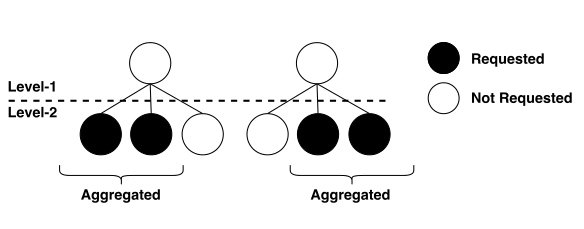
\includegraphics[scale=0.4]{Figs/tree.png}
% \caption{A Practical Request Scenario in the Hierarchical Setting}
% \label{fig:agg}
% \end{figure}
% 
% Although the two-tier scheme has a two level hierarchy (with each of the $M$ parallely executing instances of the basic scheme representing a node in the top level and the actual ciphertext classes representing nodes in the lower level), it avoids the pitfalls of existing hierarchical encryption based schemes \cite{akl1983cryptographic,ateniese2012provably}. In standard tree based hierarchical systems, granting access to the key corresponding to any node implicitly grants access to all the keys in the subtree rooted at that node. This means granting access to a selected set of nodes in a given subtree would blow up the key-size to be the same as the number of nodes. This is avoided in our two-tier scheme, since any number of nodes (ciphertext classes) that belong to the same instance may be aggregated into a single key. Figure \ref{fig:agg} summarizes this phenomenon. In the situation depicted, a tree-based hierarchy system would require $4$ decryption keys, while our 
% scheme would require only $2$. In this respect, our scheme has similar advantages to that of \cite{chu2014key}.
% 
% 
% 
% 
% 
% 
% 
% 
% 
% 
% 
